\subsection{MQTT v3.1.1}

\begin{frame}{\href{https://docs.oasis-open.org/mqtt/mqtt/v3.1.1/os/mqtt-v3.1.1-os.html}{MQTT v3.1.1} fully compliant} {Application Protocols}
  \begin{center}
    \begin{figure}
      \par\bigskip
      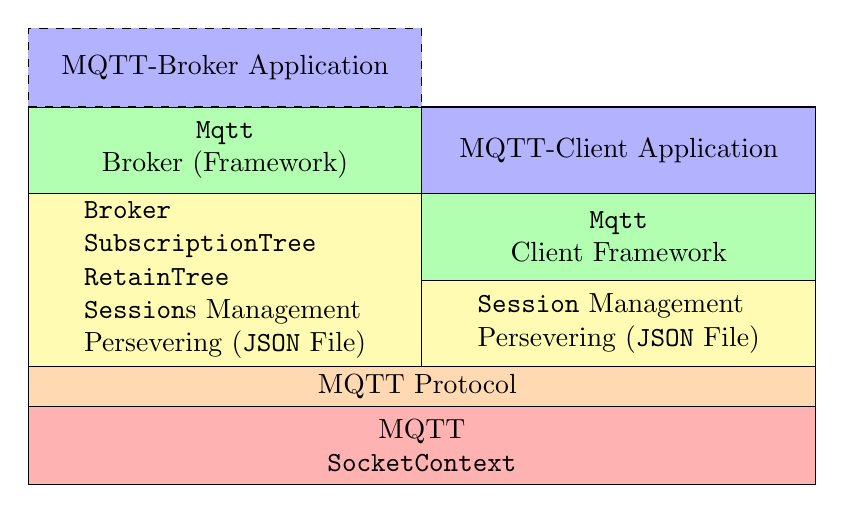
\begin{tikzpicture}
        \draw node[anchor=east, outer sep=0, inner sep=0, fill=red!30, draw, minimum width=10cm, minimum height=1cm, align=center] (wss) {MQTT \\\texttt{SocketContext}};

        \draw (wss.north) node [anchor=south, draw, outer sep=0, inner sep=0, fill=orange!30, minimum width=10cm, minimum height=0.5cm, align=center] (mqtt) {MQTT Protocol };

        \draw (mqtt.north west) node [anchor=south west, outer sep=0, inner sep=0, draw, fill=yellow!30, minimum width=5cm, minimum height=2.2cm, align=flush left] (broker) {\texttt{Broker}\\\texttt{SubscriptionTree}\\\texttt{RetainTree}\\\texttt{Session}s Management\\Persevering (\texttt{JSON} File)};

        \draw (broker.north west) node [anchor=south west, draw, outer sep=0, inner sep=0, minimum width=5cm, minimum height=1.1cm, fill=green!30, align=center] (mqtts) {\texttt{Mqtt}\\Broker (Framework)};

        \draw (mqtts.north west) node[anchor=south west, outer sep=0, inner sep=0, fill=blue!30, draw, dashed, minimum width=5cm, minimum height=1cm, align=center] (sp) {MQTT-Broker Application};

        \draw (mqtt.north east) node [anchor=south east, outer sep=0, inner sep=0, draw, fill=yellow!30, minimum width=5cm, minimum height=1.1cm, align=flush left] (client) {\texttt{Session} Management\\Persevering (\texttt{JSON} File)};

        \draw (client.north east) node [anchor=south east, draw, outer sep=0, inner sep=0, minimum width=5cm, minimum height=1.1cm, fill=green!30, align=center] (mqttc) {\texttt{Mqtt}\\Client Framework};

        \draw (mqttc.north east) node [anchor=south east, outer sep=0, inner sep=0, fill=blue!30, draw, minimum width=5cm, minimum height=1.1cm] {MQTT-Client Application};
      \end{tikzpicture}
      \caption{MQTT \texttt{SocketContext} in detail}
    \end{figure}
  \end{center}
\end{frame}
